Stochastic Gradient Descent (SGD) is used ubiquitously for minimizing neural network loss functions. SGD is an iterative 
method which is a stochastic approximation of standard gradient descent. SGD tends to achieve faster computation time of 
iterations at the expense of a slower convergence rate. In the standard gradient descent algorithm, the gradient of the
objective function is computed over the entire domain  of data points, whereas SGD approximates the gradient by computing
the gradient over a randomly sampled subset of the domain. With standard gradient descent, our problem may look like

\begin{align*}
    \text{minimize} \hspace{1em} f(x) = \frac{1}{2}\sum_{i \in D} \|N(x) - y_i \|^2
\end{align*}

where $N(x)$ is the neural network approximation and $y_i$ is the measured data. The associated update step is given by

$$
x_{k+1} = x_k - \alpha \nabla f(x)
$$

With SGD, we restrict our attention to $i \in S \subset D$ so that the update step becomes

$$
x_{k+1} = x_k - \alpha \nabla f_i(x)
$$

\noindent where $\nabla f_i(x)$ is the estimated gradient of $f$ over a domain sample.

We utilize the Adam SGD algorithm to narrow our initial search for a minimizer. Adam (Adaptive Moment Estimation) is a 
variation of traditional SGD which runs averages with exponential \say{forgetting} of both gradients and second moments
of gradients. Given parameters $w^{(t)}$ and a loss function $L^{(t)}$ with $t$ indexing the current training iteration 
starting from 0, the Adam parameter update is given in Figure \ref{fig:adam_algorithm},

\begin{figure}[H]
    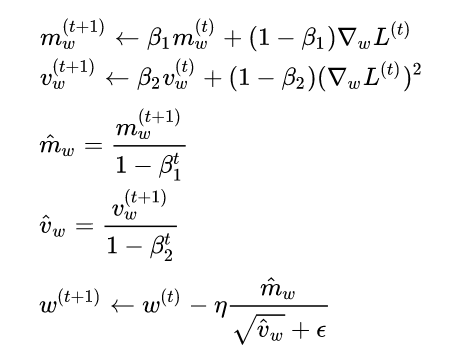
\includegraphics[width=0.40\textwidth]{images/adam.png}
    \centering
    \caption{Outline of the Adam stochastic gradient descent algorithm. Taken from Wikipedia.}
    \label{fig:adam_algorithm}
\end{figure}

where $\epsilon$ is small ($\sim10^{-8})$ and $\beta_1$ ($\sim0.9$) and $\beta_2$ ($\sim0.999$) are called the forgetting factors for the gradients and second moments of the gradients. The square root and squaring operations are done elementwise. 